\documentclass[pflichtenheft.tex]{subfiles}

\begin{document}

\chapter{Graphische Benutzeroberfläche}
Auf den Endgeräten wird eine Grafische Benutzeroberfläche angezeigt. Diese wird soll sich je nach Endgerät nur im verfügbaren Platz aufgrund der Größe der Displays unterscheiden, nicht aber in Funktionalität.

Der Nutzer soll GUI Instrumente anzeigen und ausblenden können. Zu den GUI Instrumenten gehören sowohl Dashes mit Realtime Info, als auch Graphen, die Aufzeichnungen von Daten in einem längeren Zeitraum visualisieren.


\section{DashBoard}

Auf dem Dashboard können diverse Live-Anzeigeelemente für verschiedene Informationen dargestellt werden. Um welche Informationen es sich handelt und wo diese wie angezeigt werden lässt sich über den Einstellungsknopf unten rechts konfigurieren.

\begin{figure}[H]
  	\begin{center}
 		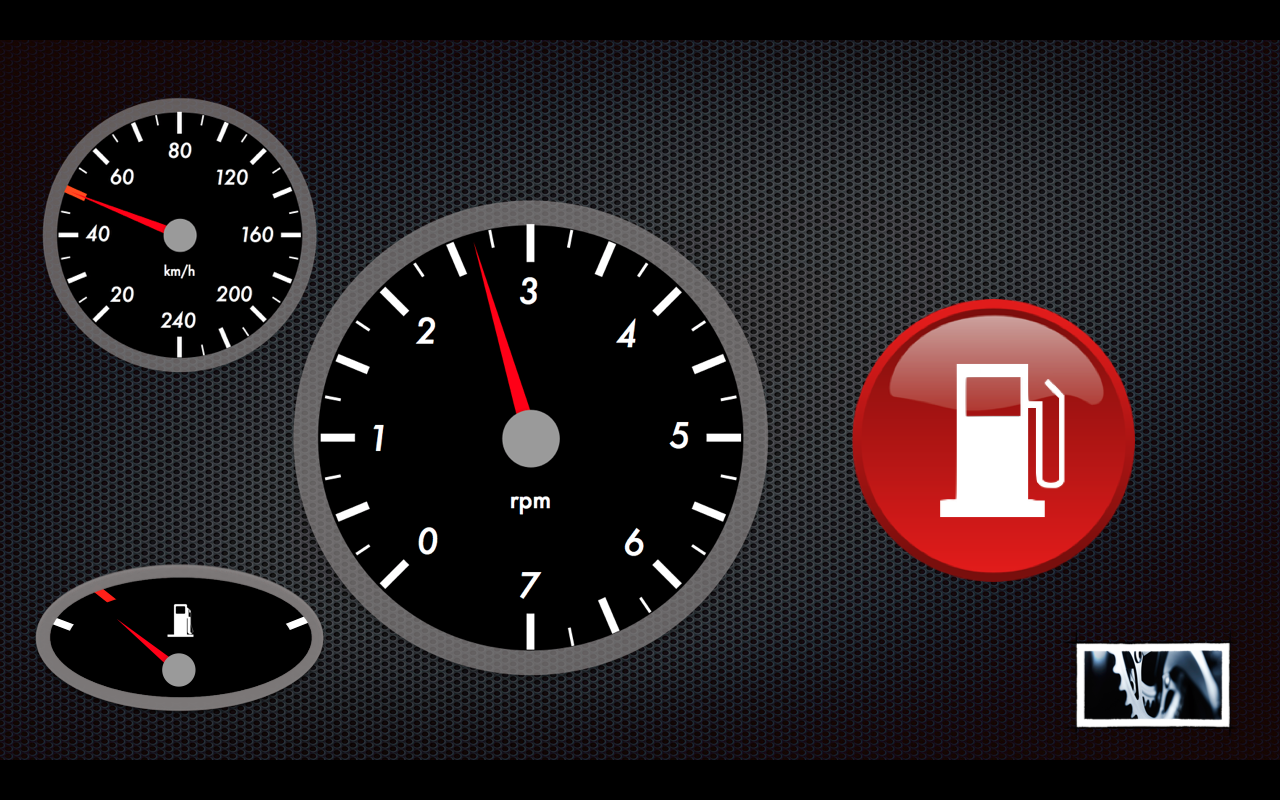
\includegraphics[width=\textwidth]{Images/GUI-Dash.png}
  		\caption{Verschiedene Dash-Anzeigeelemente.}
  	\end{center}
\end{figure}


\section{Dashboard mit Statistik}

Weitere mögliche Anzeigeelemente neben Live-Anzeigen sind Graphen auf denen Statistiken eines Wertes angezeigt werden können. Auch hier ist es möglich einzustellen um welche Informationen es sich handelt und wo diese Statistiken angezeigt werden.
\begin{figure}[H]
  	\begin{center}
 		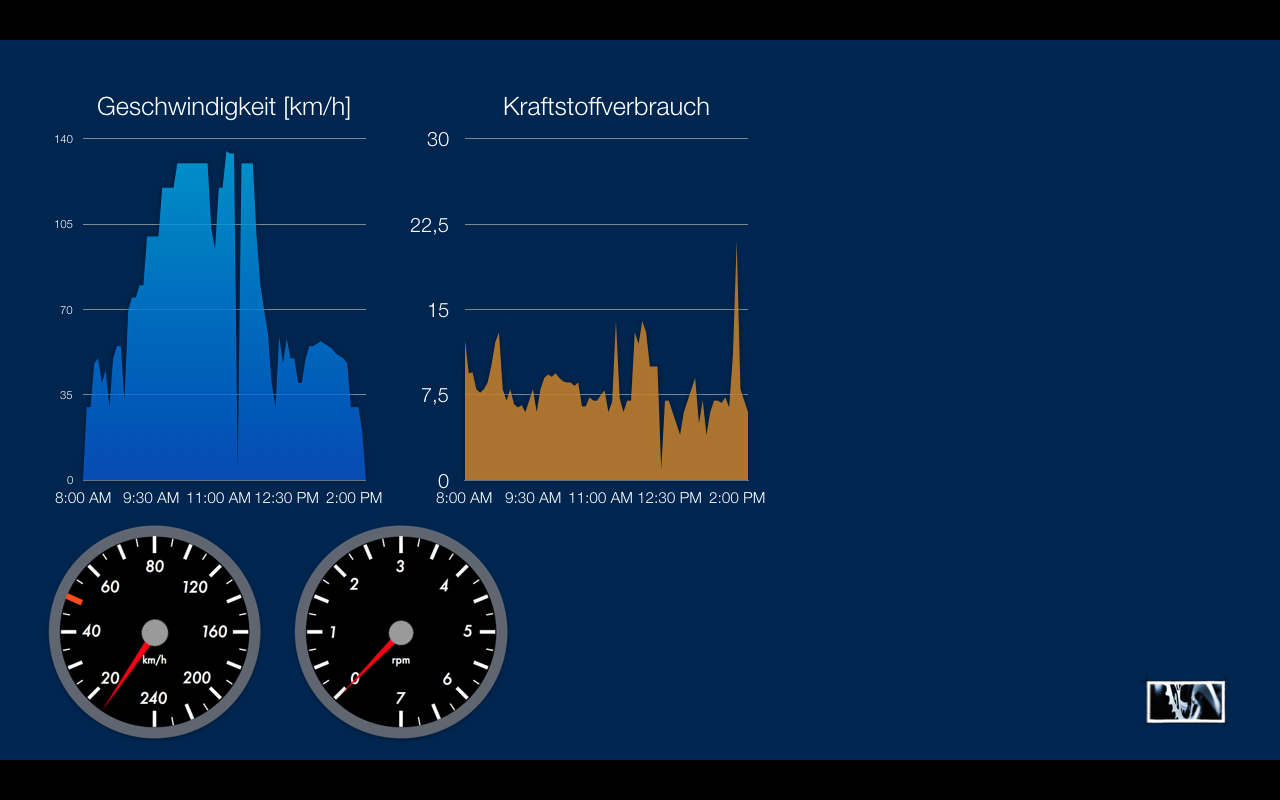
\includegraphics[width=\textwidth]{Images/GUI-DashStatistic.png}
  		\caption{Statistiken mit anderen Anzeigeelementen.}
  	\end{center}
\end{figure}

\clearpage
\section{Tabelle}

Die Tabelle, kann in verschiedenen Anzeigen genutzt werden. Die Tabellengröße, also die Anzahl der Spalten und Zeilen, ist variabel. In der Tabelle kann man scrollen und ihre Zellen können mit verschiedenen Elementen, wie z.B. Bildern oder Text gefüllt werden. Bei Berührung einer Zeile kann eine Funktion aufgerufen werden.\\
Siehe z.B. ~\nameref{sec:Karte}

\begin{figure}[H]
  	\begin{center}
 		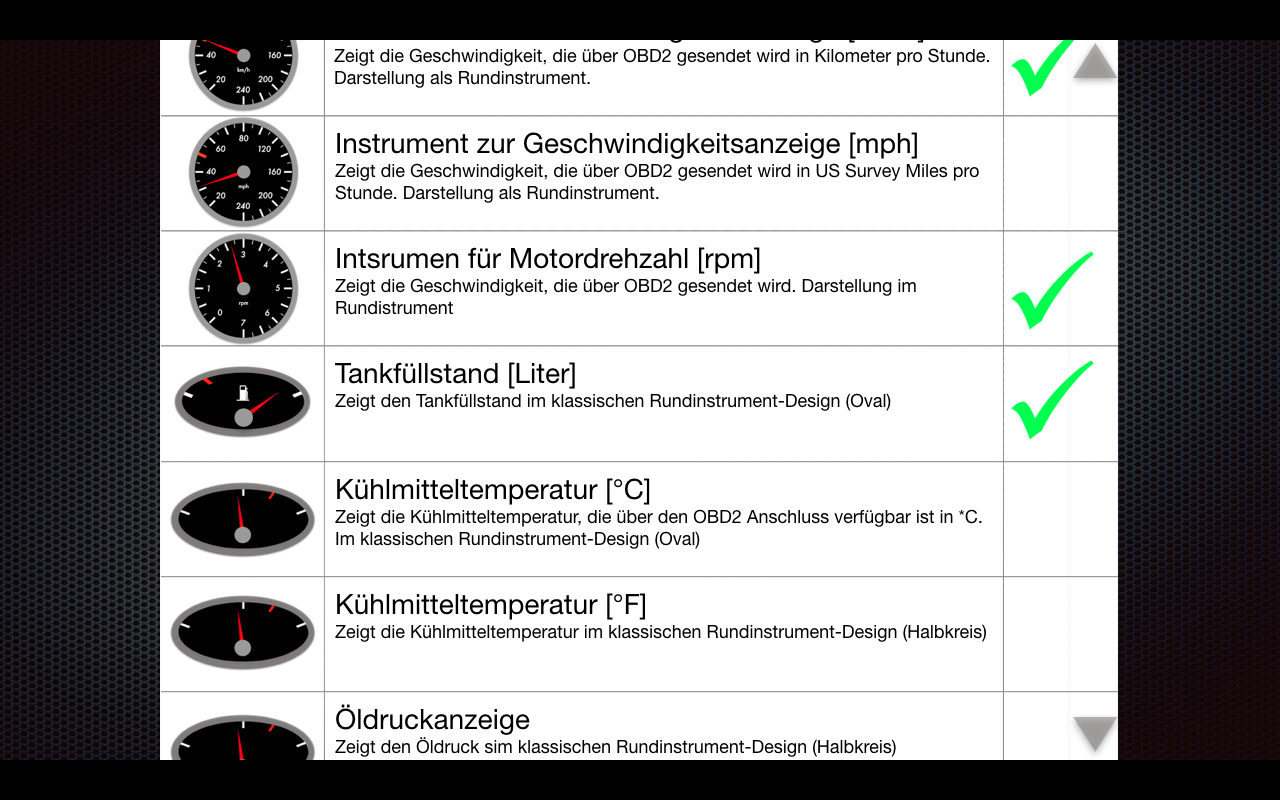
\includegraphics[width=\textwidth]{Images/GUI-Table.png}
  		\caption{Eine Beispieltabelle mit den verschiedenen verfügbaren Informationen.}
  	\end{center}
\end{figure}

\clearpage
\section{Karte}
\label{sec:Karte}

Eine weitere Ansicht ist die der Karte. Hier wird links eine Tabelle genutzt um z.B. Werkstätten oder Tankstellen in der Nähe vorzuschlagen. Links werden diese dann in einer Karte zusammen mit dem aktuellen Standort angezeigt.

\begin{figure}[H]
  	\begin{center}
 		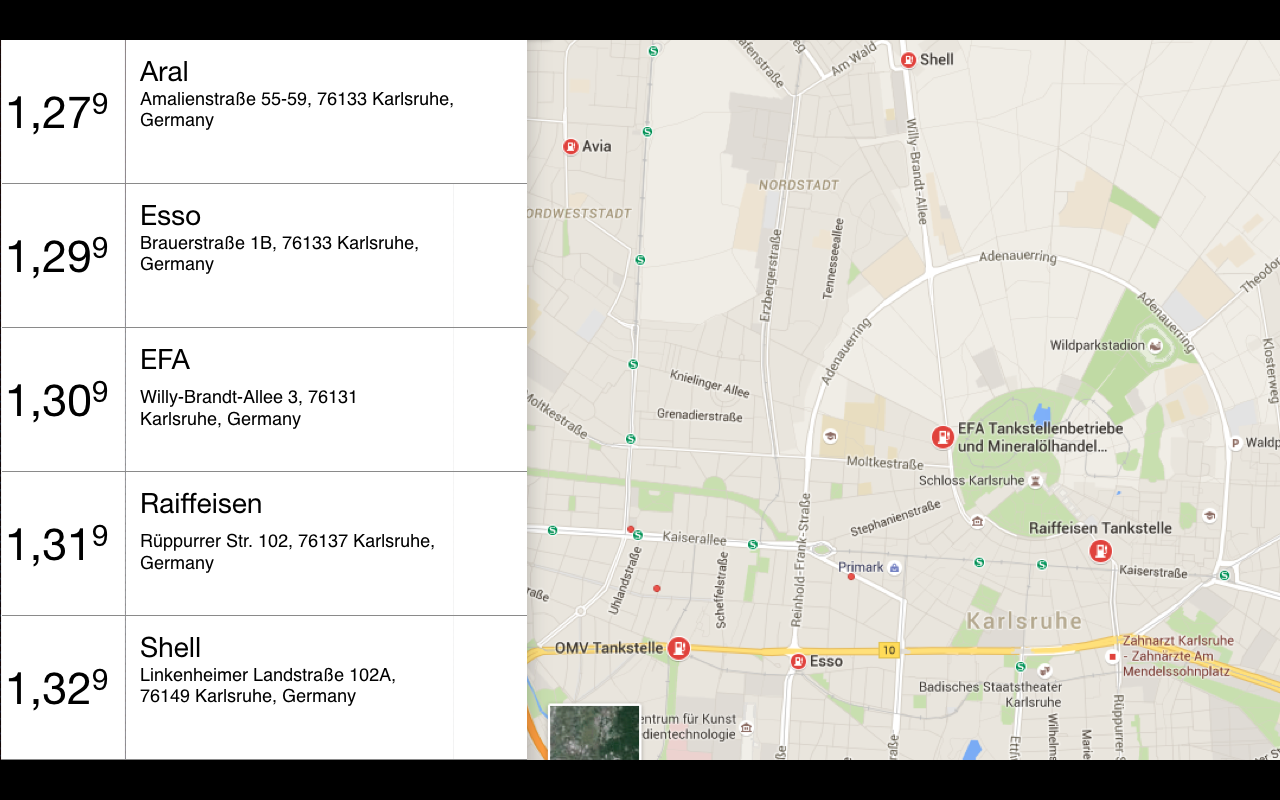
\includegraphics[width=\textwidth]{Images/GUI-Map.png}
  		\caption{Eine Kartenanzeige mit einer Tabelle}
  	\end{center}
\end{figure}


\end{document}